\subsection{Timescale}

\begin{figure}[h]
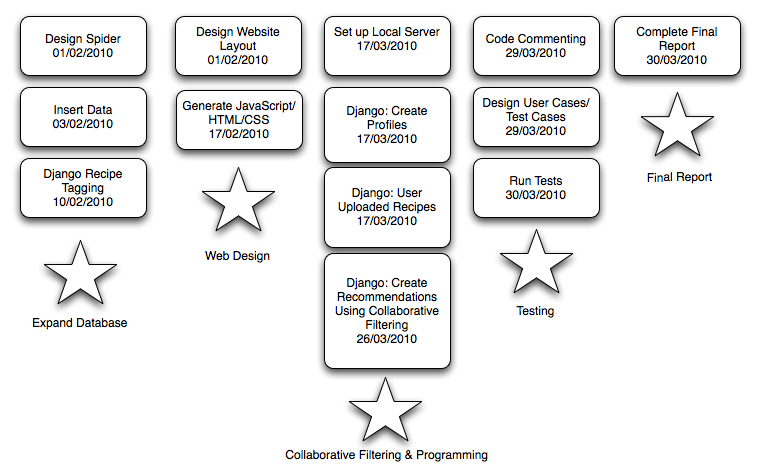
\includegraphics[width=1.1\textwidth]{milestone}
\caption{Project Timescale}
\label{fig:milestone}
\end{figure}

The project timeline can be decomposed to 4 key deadlines:
\begin{enumerate}
	\item Interim report submission (04/12/2009)
	\item Final report due (01/04/2010)
	\item Open day (05/05/2010)
	\item Presentation day (07/05/2010)

\end{enumerate}

Since our group is adopting the methodology of prototyping, a milestone chart is to be made for each of the three versions which conform to the above deadlines. Above is the detailed timeline of the version 2/3 prototype expressed as a project milestone chart (Fig~\ref{fig:milestone}). 
Each oval represents a downward progression to the milestones, represented by stars. The dates represent the deadlines that the group deemed appropriate for each progression.
For this version the group focused on designing a clean, attractive and user-friendly web interface taking into consideration simple design principles. This version also introduces the use of JavaScript and Collaborative Filtering.  Thereafter, tasks will be allocated to each member where the individual heads of the project will take charge of their respective domains. Deadlines of specific tasks are as elucidated by the above. Notice that version 2/3 is to be completed before the deadline for the final report which exemplifies the fact that our chart takes into account the major deadline dates.

\newpage

 
